\documentclass{scrartcl}
\usepackage[utf8]{inputenc}
\usepackage{hyperref}
\usepackage{url}
\usepackage{natbib}
\usepackage{graphicx}
\usepackage{enumitem}
\usepackage{cleveref}
%% for labeling items
\renewcommand\labelenumi{\arabic{enumi}.}
\renewcommand\theenumi{\thesubsection.\arabic{enumi}}%% references with subsection numbering

\newcommand{\emailaddr}[1]{\href{mailto:#1}{\texttt{#1}}}

\title{
    Revue
}


\author{
    Mattia Matteini \\ \emailaddr{mattia.matteini@studio.unibo.it}
    \and
    Alberto Paganelli \\ \emailaddr{alberto.paganelli3@studio.unibo.it}
}

\date{March 2023}

\begin{document}

    \maketitle

    \begin{abstract}
        Revue is a real-time video surveillance and environment monitoring system. It is designed to be used in multiple scenarios such as home, office or warehouses following the user needs.
%
        Composed by multiple features, it permits high modularity, allowing a more complex usage through the video streaming detection of predefined set of object classes and sending alerts to the user or simply to monitoring camera streams.
    \end{abstract}


    \section{Requirements}

    The goal of the project is to develop a distributed software system which is able to monitor the environment
    of a certain area through sensors and cameras, providing real-time data and video streaming.

    Moreover, to enhance the usefulness of the system, it should also be able to notify the user when specificconditions are met.
    These conditions include detecting if sensor data exceeds a predetermined range or if the camerarecognises a particular object.
    This notification feature ensures that the user is promptly informed about critical
    events or anomalies in the monitored environment.

    The outcome should be a reliable system adaptable to different scenarios, such as smart cities, industrial, or
    simply home monitoring.

    In the following are listed the main requirements of the system.

    \subsection{User Requirements}\label{subsec:user-requirements}

    \begin{enumerate}
        \item \label{itm:user-1} The user can authenticate to the system through a web interface.
        \item \label{itm:user-2} The user can monitor the environment data produced by the sensors.
        \item \label{itm:user-3} The user can monitor the video stream produced by the cameras.
        \item \label{itm:user-4} The user can add/delete a device to the system.
        \item \label{itm:user-5} The user can enable and disable a device.
        \item \label{itm:user-6} The user can modify a device configuration.
        \item \label{itm:user-7} The user can add/delete a security rule regarding a camera/sensor.
        \item \label{itm:user-8} The user can modify a security rule.
        \item \label{itm:user-9} The user can delete received notifications.
        \item \label{itm:user-10} The user can consult the history of produced data.
    \end{enumerate}

    \subsection{System Requirements}\label{subsec:system-requirements}
    \begin{enumerate}
        \item \label{itm:sys-1} The system grants access only to authenticated users.
        \item \label{itm:sys-2} The system provides a web interface as an entry point for the user.
        \item \label{itm:sys-3} The system generates video and data streams.
        \item \label{itm:sys-4} The system monitors streams in order to detect anomalies.
        \item \label{itm:sys-5} The system notifies the user when a security rule is violated.
        \item \label{itm:sys-6} The system persistently stores produced data.
    \end{enumerate}

    \subsection{Non-functional Requirements}\label{subsec:non-functional-requirements}
    \begin{enumerate}
        \item \label{itm:func-1} The system should work even though the recognition component is down or not deployed.
        \item \label{itm:func-2} The system should work even though the component responsible for the storage of the data is down or not deployed.
        \item \label{itm:func-3} The system should be replicable in order to increase the availability of the system.
        \item \label{itm:func-4} The system should work even though the component responsible for the authentication is down.
        \item \label{itm:func-5} The video compartment should be independent of the data compartment and vice versa.
    \end{enumerate}

    \subsection{Implementation Requirements}\label{subsec:implementation-requirements}
    \begin{enumerate}
        \item \label{itm:impl-1} The recognition component of the system should be implemented in Python.
        \item \label{itm:impl-2} The frontend of the system should be implemented using Vue 3 and Typescript.
        \item \label{itm:impl-3} The storage of data should be implemented using a NoSQL database.
        \item \label{itm:impl-4} The system should be implemented using a microservices architecture.
        \item \label{itm:impl-5} The system should be deployed using Docker.
    \end{enumerate}

    \subsection{Scenarios}
    The system can be used in various scenarios, depending on the user needs.
    This system is designed to be used by multiple types of users, from a private user to a company director.
    In the sections below, we will describe two main of the possible scenarios in which the system can be used.

    In the simplest scenario, the system is used by a private user, who wants just to monitor his home or a particular environment without the necessity
    to recognise the objects in the video. In this case, the user can just rely on the camera, monitoring the home or a proprietary field. The user is free to monitor the live video by the camera whenever and wherever he/she wants, using the browser on the smartphone.
    The user can also set up sensors to monitor data from the environment.

    \begin{figure}
        \centering
        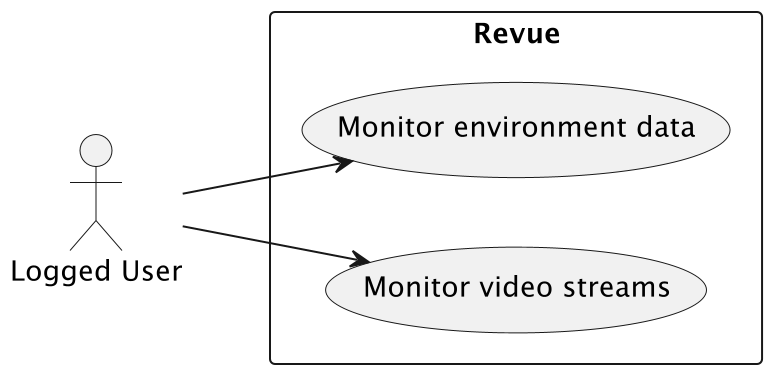
\includegraphics[scale=0.6]{img/simple-use-case}
        \caption{Simple Use Case}
        \label{fig:simple-use-case}
    \end{figure}

    A more complex scenario could involve both sensor and camera usages with the support of a neural network to detect intrusion. For example, the director of food wholesale could
    monitor the temperature of the warehouse and the presence of unauthorised people during the night. In this case, the
    recognition part of the system is necessary to detect whenever an intrusion occurs.
    Moreover, supply chain monitoring can be done for who's needs to ensure that the temperature of
    the warehouse is always in the right range and be alerted whenever the temperature exceeds a certain range to detect or
    prevent problems.

    \begin{figure}
        \centering
        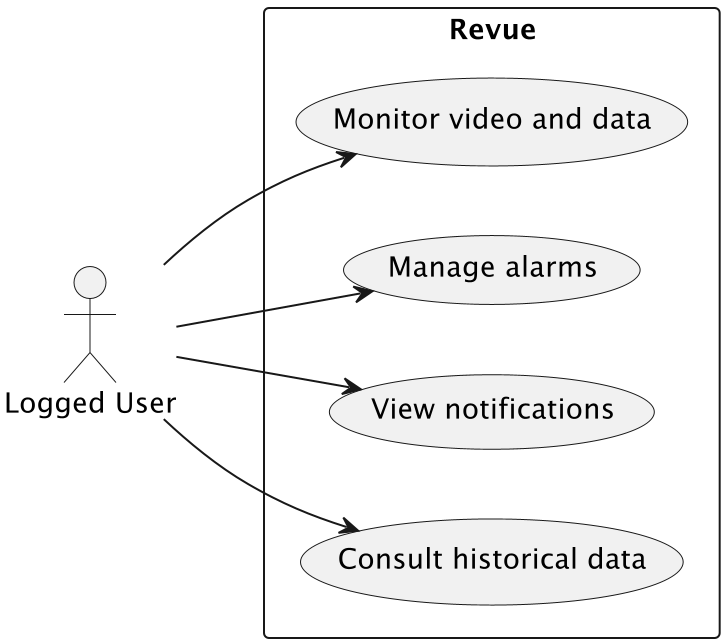
\includegraphics[scale=0.6]{img/advanced-use-case}
        \caption{Advanced Use Case}
        \label{fig:advanced-use-case}
    \end{figure}

    \subsection{Self-assessment policy}

    The project can be considered completed when \textbf{all} requirements are satisfied.

    In particular, non-functional requirements aim to grant a good general quality of the system. This will be achieved also using automated tests that will ensure, among other things, the quality code production.


    \section{Requirements Analysis}

%Is there any implicit requirement hidden within this project's requirements?
%
%Is there any implicit hypothesis hidden within this project's requirements?
%
%Are there any non-functional requirements implied by this project's requirements?

%What model / paradigm / techonology is the best suited to face this project's requirements?
%
%What's the abstraction gap among the available models / paradigms / techonologies and the problem to be solved?

    Drawing up requirements, one relevant thing considered is the recognition feature. This is supposed to be developed using Python and exploiting its main libraries for video processing and object recognition, in order to minimise the abstraction gap.

    Another important aspect is the handling of video streams. In fact, to facilitate development, an implicit requirement is necessary: the use of an ad hoc \textit{media server}. This permits also to improve the compatibility permitting to produce and consume using different protocols.

    Eventually, internal communications between devices and services need to be guaranteed. This implicitly leads to the use of a message broker (\textit{Kafka}) which guarantees better scalability and at least one message delivery policy.


    \section{Design}

% This is where the logical / abstract contribution of the project is presented.

% Notice that, when describing a software project, three dimensions need to be taken into account: structure, behaviour, and interaction.

% Always remember to report \textbf{why} a particular design has been chosen.
% Reporting wrong design choices which has been valued during the design phase is welcome too.

    \subsection{Architecture}

    The overall system is designed with microservices architecture.
%
    This choice helped us to increase modularity, scalability, reliability and fault tolerance.

    The system is composed of the following microservices:
    \begin{itemize}
        \item \textbf{Authentication Service}: responsible for the authentication and access control.
        \item \textbf{Monitoring Service}: responsible for managing devices and environment data.
        \item \textbf{Recognition Service}: responsible for the recognition of objects in the video streams.
        \item \textbf{Alarm Service}: responsible for the management of the security rules and anomalies.
        \item \textbf{Notification Service}: responsible for sending notifications to the user.
        \item \textbf{Log Service}: responsible for the persistent saving of data.
    \end{itemize}

    Each microservice consists of a web server that exposes REST APIs and a database to store the data (Figure \ref{fig:microservice}).

    \begin{figure}
        \centering
        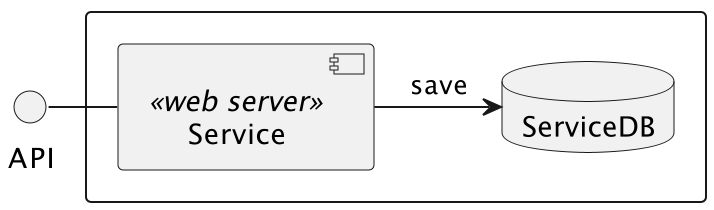
\includegraphics[scale=0.6]{img/microservice}
        \caption{Microservice components}
        \label{fig:microservice}
    \end{figure}

    Moreover, other components are necessary to make the system work:

    \begin{itemize}
        \item \textbf{Frontend}: provides to the user the web interface to interact with the system.
        \item \textbf{Sensors}: capture the environment data and send them to the rest of the system.
        \item \textbf{Cameras}: capture the video streams and send them to the rest of the system.
        \item \textbf{Media Server}: used to consume the produced video streams and make them available using different protocols.
        \item \textbf{Broker}: used to manage some internal communications.
    \end{itemize}

    \begin{figure}
        \centering
        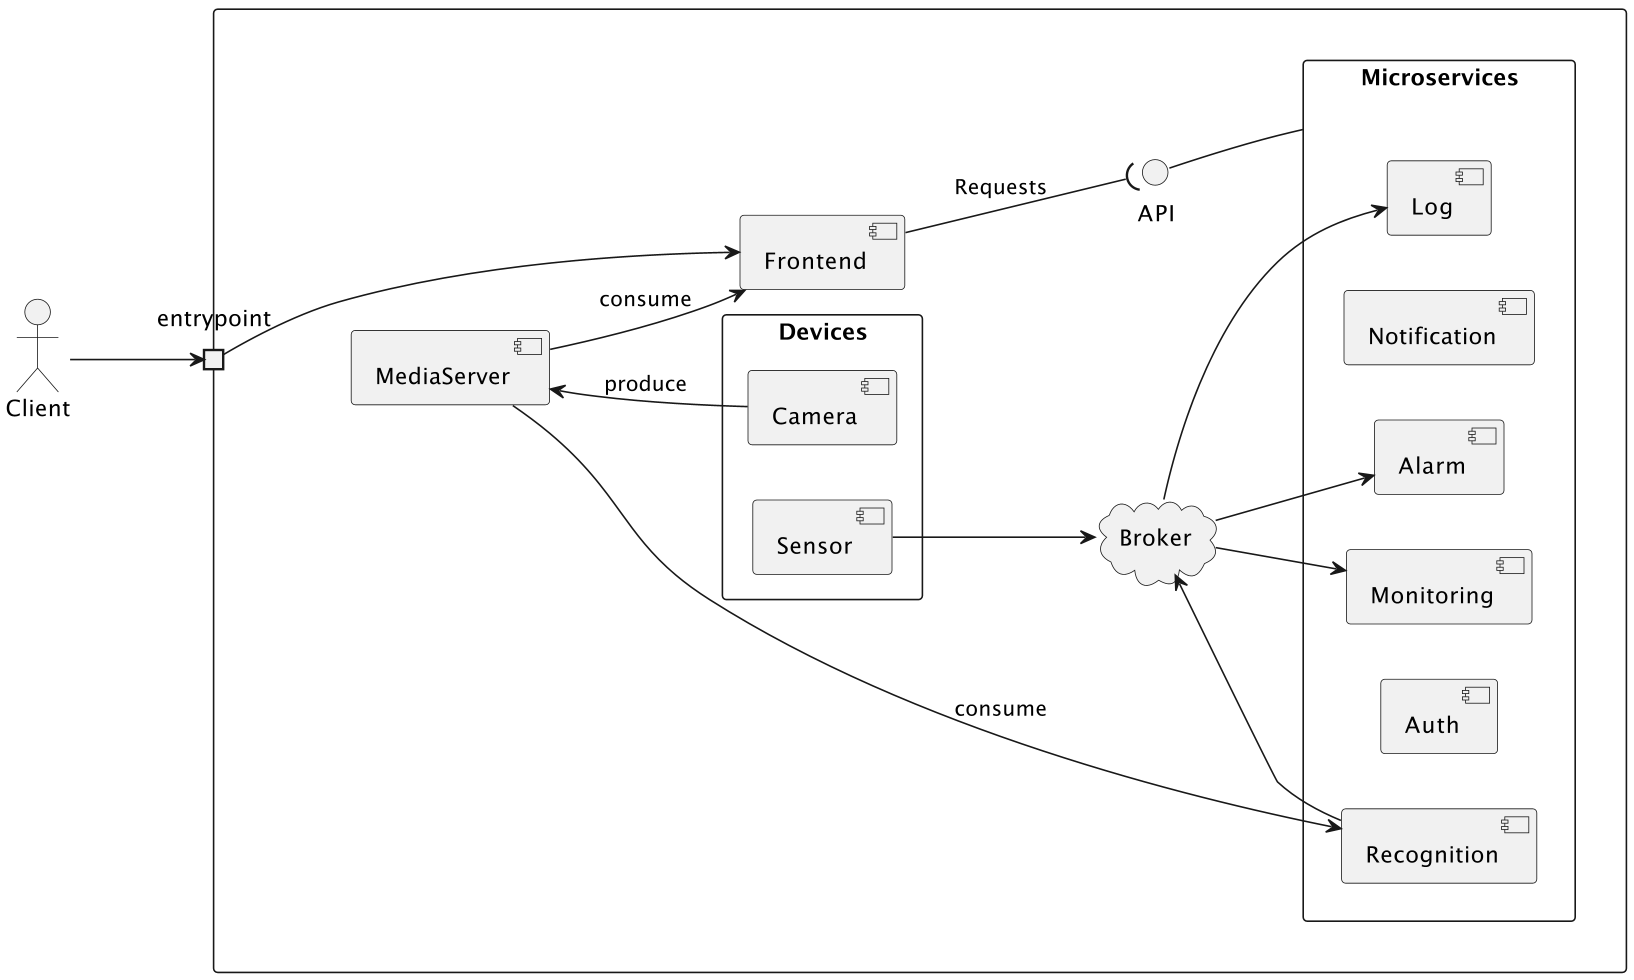
\includegraphics[scale=0.51]{img/architecture}
        \caption{Revue Architecture}
        \label{fig:architecture}
    \end{figure}


    \subsection{Structure}

    Which entities need to be modelled to solve the problem?
%
    (UML Class diagram)

    How should entities be modularised?
%
    (UML Component / Package / Deployment Diagrams)


    \begin{figure}
        \centering
        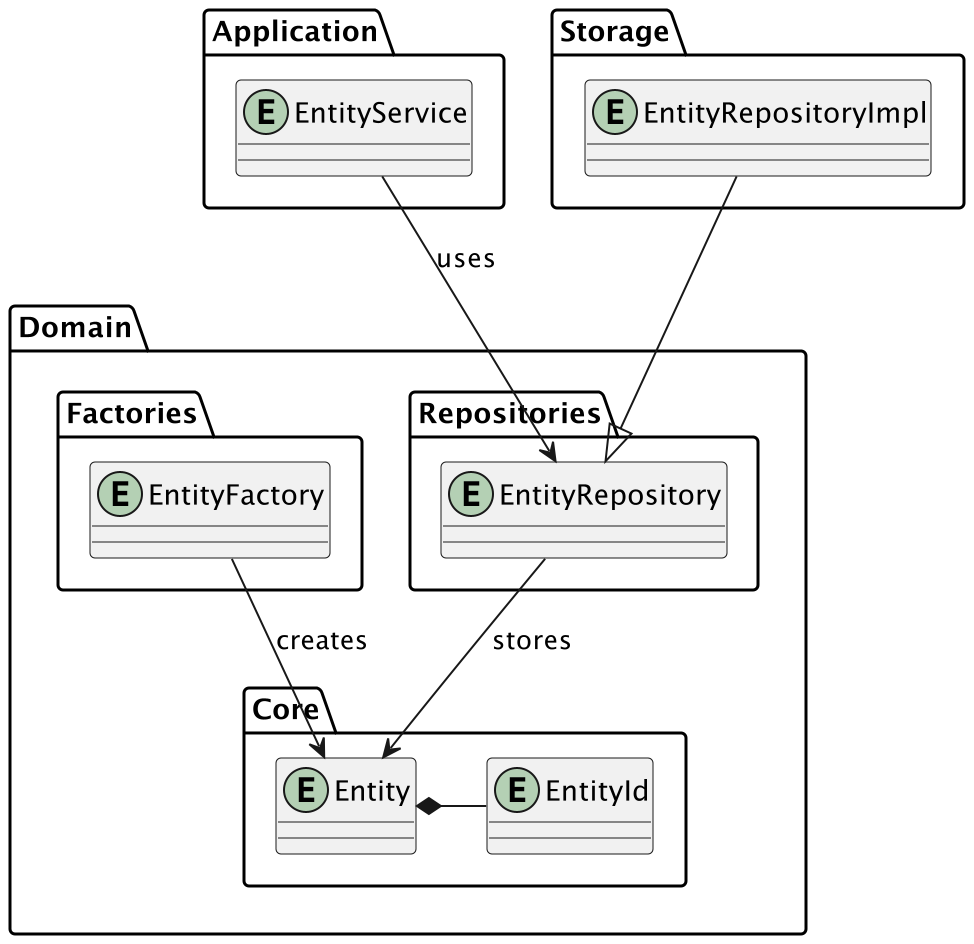
\includegraphics[scale=0.55]{img/general-structure}
        \caption{General structure of microservice}
        \label{fig:general-structure}
    \end{figure}

    \subsection{Behaviour}

    \subsubsection{Authentication Service}

    \subsubsection{Monitoring Service}
    \begin{figure}
        \centering
        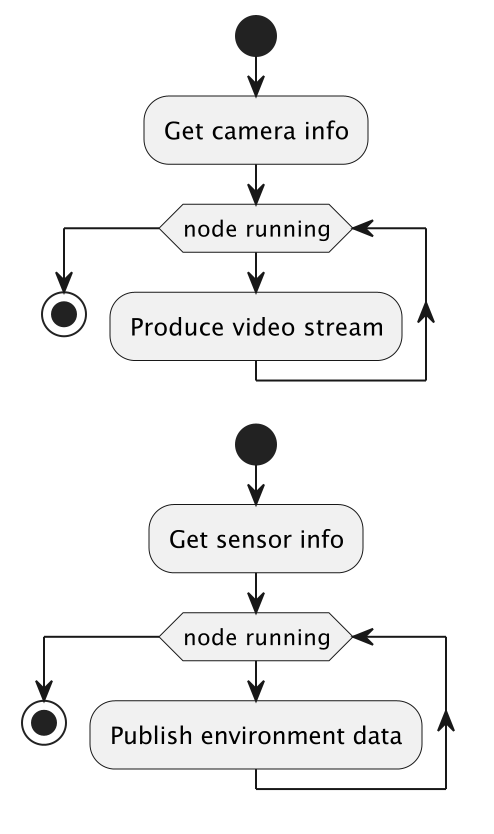
\includegraphics[scale=0.4]{img/device-activity}
        \caption{Device activity diagram}
        \label{fig:device-activity}
    \end{figure}

    \subsubsection{Recognition Service}
    \begin{figure}
        \centering
        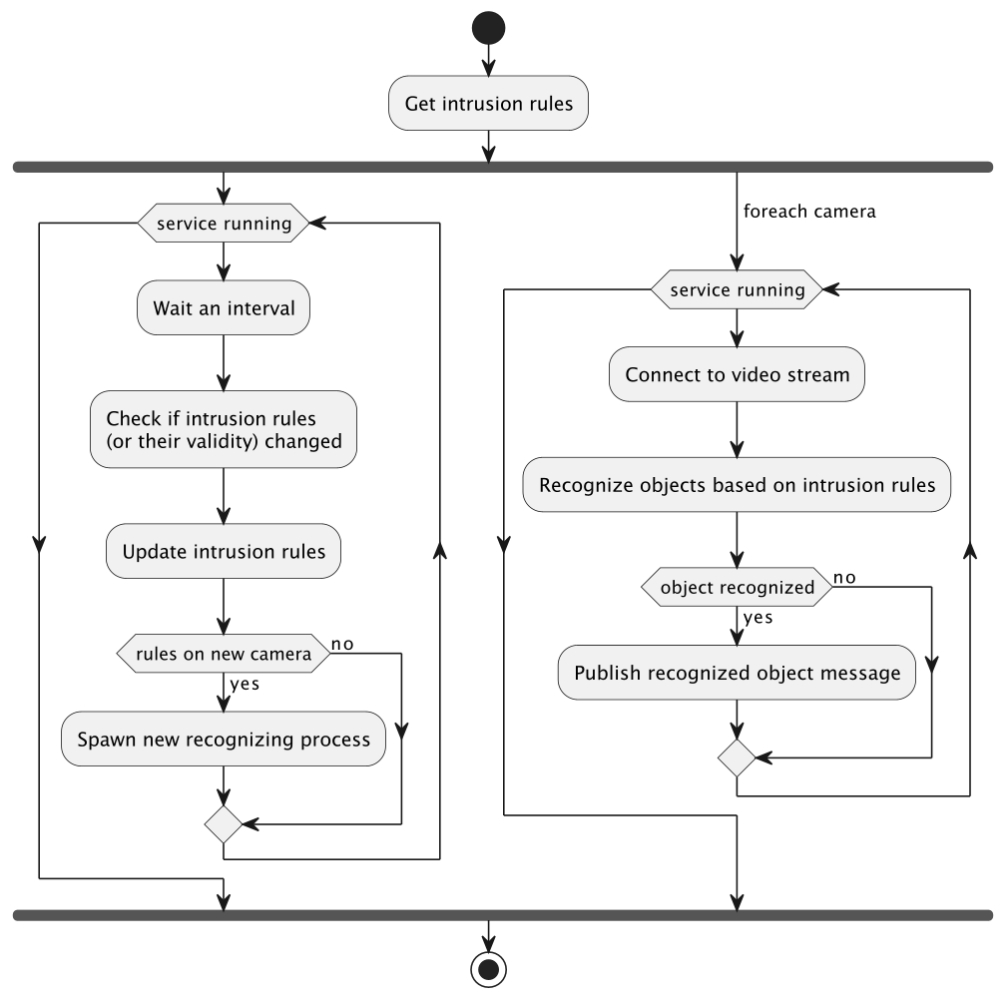
\includegraphics[scale=0.6]{img/recognition-activity}
        \caption{Recognition service activity diagram}
        \label{fig:recognition-activity}
    \end{figure}
    Microservice responsible of the recognition of the objects on the camera streams. The service is able to recognize a set of predefined objects and notify the Alarm Service that is in charge of the alarm management. For every camera stream a topic and a recognition process is created and started. When a predefined object is recognized it is sent trought the relative topic.


    \subsubsection{Alarm Service}
    \begin{figure}
        \centering
        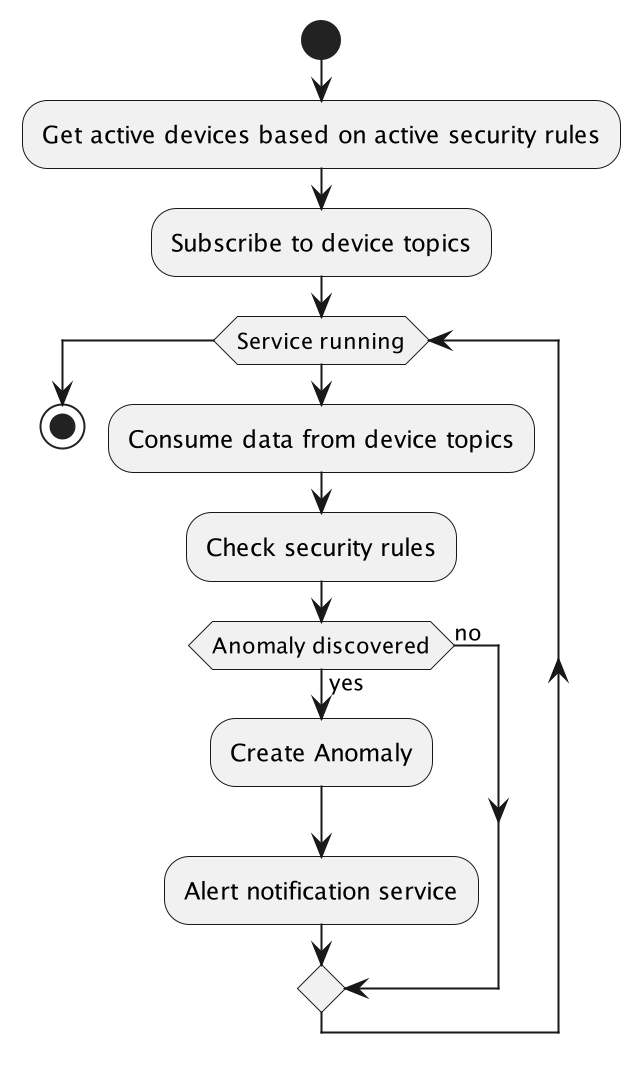
\includegraphics[scale=0.3]{img/alarm-activity}
        \caption{Alarm service activity diagram}
        \label{fig:alarm-activity}
    \end{figure}
    Microservice responsible of the alarm management. It is able to check the data coming from the sensors or the recognized objects on cameras streams. The service needs only to check active rules for active devices. It is able to create an anomaly and to notify the notification service if the data is not compliant with the rules.

    \subsubsection{Notification Service}

    \subsubsection{Log Service}


    \subsection{Interaction}

    \subsubsection{Auth Service}
    \begin{figure}
        \centering
        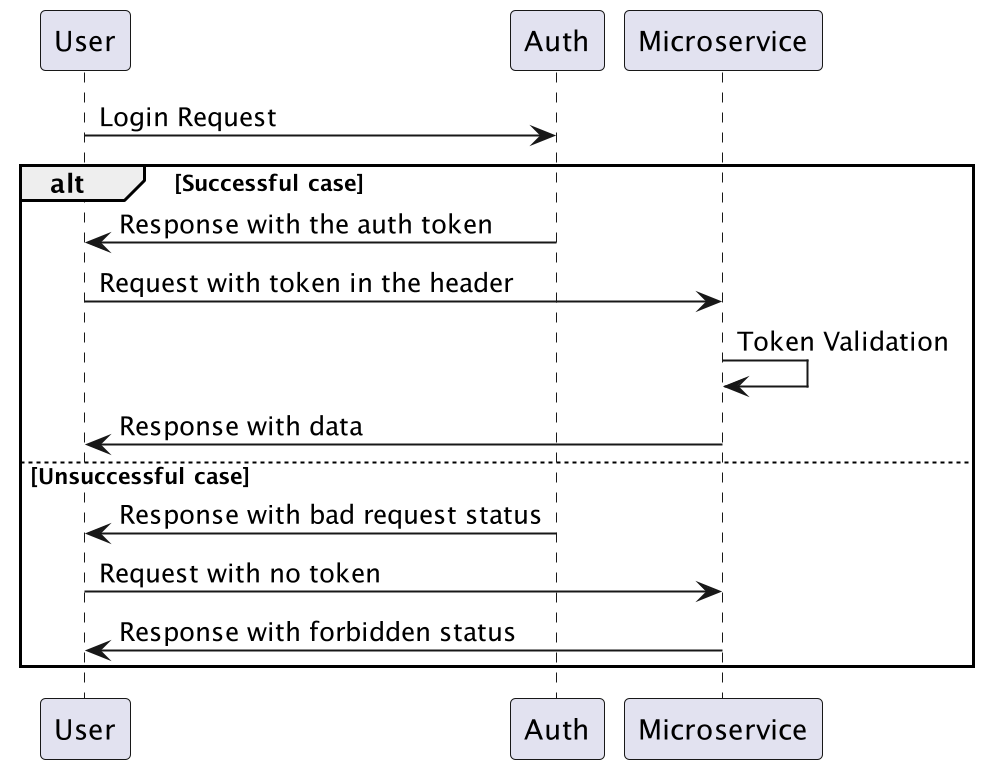
\includegraphics[scale=0.3]{img/auth-service-sequence}
        \caption{Auth service sequence diagram}
        \label{fig:auth-service-sequence}
    \end{figure}
    The Auth Service is responsible of the authentication of the users. When a Login request is performed, the Auth Service checks the credentials and returns a token if the user is authenticated. When the user wants to perform a request to another service, the user needs only to provide the token in the header of the request. Every service contains a validation middleware where the token is checked. This process has been implemented through the use of JSON Web Token and sharing the secret key between federated services.

    How should entities interact with each other?
%
    (UML Sequence Diagram)


    \section{Implementation Details}

    Just report interesting / non-trivial / non-obvious implementation details.

    This section is expected to be short in case some documentation (e.g. Javadoc or Swagger Spec) has been produced for the software artefacts.
%
    This this case, the produced documentation should be referenced here.

    \begin{itemize}
        \item Kafka publish/subscription - Kafka per il real time e reliability (at least one)
        \item Recognition neural network
        \item Media server
        \item Socket per comunicazione real time al client
        \item SSO
    \end{itemize}


    \section{Self-assessment / Validation}

    Choose a criterion for the evaluation of the produced software and \textbf{its compliance to the requirements above}.

    Pseudo-formal or formal criteria are preferred.

    In case of a test-driven development, describe tests here and possibly report the amount of passing tests, the total amount of tests, and possibly the test coverage.

    \begin{itemize}
        \item architecture tests
        \item fault tolerance test
        \item prettier e linter
    \end{itemize}

    \section{Deployment Instructions}

    Explain here how to install and launch the produced software artefacts.
%
    Assume the softaware must be installed on a totally virgin environment.
%
    So, report \textbf{any} configuration step.

    Gradle and Docker may be useful here to ensure the deployment and launch processes to be easy.


    \section{Usage Examples}

    For every usage, the system require a login for security reasons.

    LOGIN PIC

    In the simplest scenario the user can see the section designated for sensor environment data or the camera video streams consultation.

    HOME PIC e CAMERA PIC

    In the more complex scenario the user can add security rules in order to detect exceeding values or unauthorized objects in the video streams.
    When adding a new security rule the user can choose the object class to detect or the threshold value (for a particular measure) in addition to the device and time slot in which the rule is active.

    SECURITY RULES PIC

    Both usage of the system consent to the user to add, delete or modify a device or a security rule configuration.

    UPDATE DEVICE E SECURITY RULES PIC

    Moreover, the user can consult the history of produced data or all the notifications received by the system.

    HISTORY PIC e NOTIFICATIONS PIC


    \section{Conclusions}

    Recap what you did

    \subsection{Future Works}

    Recap what you did \emph{not}

    \subsection{What did we learned}

    Racap what did you learned

    \section*{Stylistic Notes}

    Use a uniform style, especially when writing formal stuff: $X$, X, $\mathbf{X}$, $\mathcal{X}$, \texttt{X} are all different symbols possibly referring to different entities.

    This is a very short paragraph.

    This is a longer paragraph (notice the blank line in the code).
    It composed by several sentences.
%
    You're invited to use comments within \texttt{.tex} source files to separate sentences composing the same paragraph.

    Paragraph should be logically atomic: a subordinate sentence from one paragraph should always refer to another sentence from within the same paragraph.

    The first line of a paragraph is usually indented.
%
    This is intended: it is the way \LaTeX{} lets the reader know a new paragraph is beginning.

    Use the \href{https://en.wikibooks.org/wiki/LaTeX/Source_Code_Listings}{\texttt{listing}} package for inserting scripts into the \LaTeX{} source.

    \nocite{*} % Includes all references from the `references.bib` file
    \bibliographystyle{plain}
    \bibliography{references}

\end{document}
